% Options for packages loaded elsewhere
\PassOptionsToPackage{unicode}{hyperref}
\PassOptionsToPackage{hyphens}{url}
\documentclass[
  11pt,
  letterpaper,
]{article}
\usepackage{xcolor}
\usepackage[left=0.82in,right=0.82in,top=0.73in,bottom=0.77in]{geometry}
\usepackage{amsmath,amssymb}
\setcounter{secnumdepth}{5}
\usepackage{iftex}
\ifPDFTeX
  \usepackage[T1]{fontenc}
  \usepackage[utf8]{inputenc}
  \usepackage{textcomp} % provide euro and other symbols
\else % if luatex or xetex
  \usepackage{unicode-math} % this also loads fontspec
  \defaultfontfeatures{Scale=MatchLowercase}
  \defaultfontfeatures[\rmfamily]{Ligatures=TeX,Scale=1}
\fi
\usepackage{lmodern}
\ifPDFTeX\else
  % xetex/luatex font selection
\fi
% Use upquote if available, for straight quotes in verbatim environments
\IfFileExists{upquote.sty}{\usepackage{upquote}}{}
\IfFileExists{microtype.sty}{% use microtype if available
  \usepackage[]{microtype}
  \UseMicrotypeSet[protrusion]{basicmath} % disable protrusion for tt fonts
}{}
\makeatletter
\@ifundefined{KOMAClassName}{% if non-KOMA class
  \IfFileExists{parskip.sty}{%
    \usepackage{parskip}
  }{% else
    \setlength{\parindent}{0pt}
    \setlength{\parskip}{6pt plus 2pt minus 1pt}}
}{% if KOMA class
  \KOMAoptions{parskip=half}}
\makeatother
\usepackage{longtable,booktabs,array}
\usepackage{caption}
\captionsetup[table]{skip=6pt}
\newcounter{none} % for unnumbered tables
\usepackage{calc} % for calculating minipage widths
% Correct order of tables after \paragraph or \subparagraph
\usepackage{etoolbox}
\makeatletter
\patchcmd\longtable{\par}{\if@noskipsec\mbox{}\fi\par}{}{}
\makeatother
\usepackage{graphicx}
\makeatletter
\newsavebox\pandoc@box
\newcommand*\pandocbounded[1]{% scales image to fit in text height/width
  \sbox\pandoc@box{#1}%
  \Gscale@div\@tempa{\textheight}{\dimexpr\ht\pandoc@box+\dp\pandoc@box\relax}%
  \Gscale@div\@tempb{\linewidth}{\wd\pandoc@box}%
  \ifdim\@tempb\p@<\@tempa\p@\let\@tempa\@tempb\fi% select the smaller of both
  \ifdim\@tempa\p@<\p@\scalebox{\@tempa}{\usebox\pandoc@box}%
  \else\usebox{\pandoc@box}%
  \fi%
}
% Set default figure placement to htbp
\def\fps@figure{htbp}
\makeatother
\setlength{\emergencystretch}{3em} % prevent overfull lines
\providecommand{\tightlist}{%
  \setlength{\itemsep}{0pt}\setlength{\parskip}{0pt}}
\usepackage{needspace}
\clubpenalty=10000
\widowpenalty=10000
\pretocmd{\section}{\Needspace{6\baselineskip}}{}{}
\pretocmd{\subsection}{\Needspace{10\baselineskip}}{}{}
\usepackage{bookmark}
\IfFileExists{xurl.sty}{\usepackage{xurl}}{} % add URL line breaks if available
\urlstyle{same}
% fallback for those not using the hyperref driver hyperxmp:
\makeatletter
\@ifundefined{xmpquote}{\newcommand{\xmpquote}[1]{#1}}{}
\makeatother
\hypersetup{
  pdftitle={Verified Prepared-Tree Replay for Package Installation},
  pdfauthor={Bhuvan Prakash · Independent Researcher},
  hidelinks,
  pdfcreator={LaTeX via pandoc}}

\title{Verified Prepared-Tree Replay for Package Installation}
\usepackage{etoolbox}
\makeatletter
\providecommand{\subtitle}[1]{% add subtitle to \maketitle
  \apptocmd{\@title}{\par {\large #1 \par}}{}{}
}
\makeatother
\subtitle{Isolated sibling refill in Jhol Instant Lock}
\author{Bhuvan Prakash · Independent Researcher}
\date{13 November 2026 · Jhol Research Series III}

\begin{document}
\maketitle

\subsection*{Abstract}\label{abstract}
\addcontentsline{toc}{subsection}{Abstract}

Prepared-tree replay can reduce the latency of repeated package
installation, but refilling a consumed snapshot from the live tree can
race user cleanup. We present a two-slot replay protocol that binds the
request identity, restores a prepared tree by rename, verifies the
resulting layout, and refills from an isolated sibling. In a bounded
model, sibling refill succeeds under all five placements of a live-tree
deletion. Live-source refill succeeds in three. On a synthetic 738-file
APFS fixture, 30 matched trials per operation give median times of 0.258
ms for rename and 11.231 ms for recursive directory cloning. Archived
Express runs additionally record the caller and worker costs of the
install path. The study separates the visibility of a restored tree,
successful layout verification, and the later cost of replenishing a
slot.

\section{Introduction}\label{introduction}

In Jhol, restoring a prepared tree was quick. Keeping a prepared tree
available for the next call was harder. A refill worker copied from the
live directory just as the next trial deleted it. That race explains why
a fast restore could alternate with a slow miss. Its contributions are a
protocol for isolated sibling refill, a safety argument for successful
replay under a stated layout contract, and an evaluation that separates
foreground publication from clone work.

\section{Background and Related Work}\label{background-and-related-work}

Bazel's remote cache separates declared action inputs from cached
outputs {[}1{]}. Nix's functional deployment model associates store
paths with declared build inputs {[}2{]}. Jhol restores a prepared
result into a mutable project path, where application processes and
later installs can observe or change it. Crash-consistency work shows
that namespace operations and data persistence depend on the filesystem
and its guarantees {[}3{]}. This distinction motivates a separate
analysis of process interruption and durable recovery.

\section{System Model}\label{system-model}

Let \(K\) denote the identity of an eligible install request. Its
components should include final manifest and supported lock bytes,
install mode and layout version, platform and policy inputs that can
change the result. Let \(A(K)\) be the layout authorized by the lockfile
and current supported policy. Define \(V_K(T)\) as a check of required
package paths and identities and of unauthorized package directories in
an installed tree \(T\). The runtime checker provides a layout verdict.
Stronger byte or provenance claims need separate integrity evidence.

Jhol's earlier JHLCPL capsule encodes a derived binary plan. It can
avoid parsing the plan while still requiring open-time bounds and string
validation, correct source selection and valid materialization. GRM is a
process-local DashMap-sharded record store. It remains in the codebase,
including spec queries used by other paths, but capsule-first warm
install keeps GRM and Soul Path off the hot path. Removing an outer
mutex does not establish wait-free or lock-free progress for operations
on sharded maps. The degree-sequence certificate estimates risk from
root specifications. It does not authorize installed-tree replay.

The prepared snapshot is a different artifact. It stores a previously
installed tree in project-local slots and removes repeat clone work from
the common restore path. Its safety depends on exactly which outputs
were validated and how they are protected from changes. Strict frozen
installs, explicit package requests, workspace links, and
lifecycle-sensitive cases require their own semantics and must use a
shortcut only when its preconditions cover them.

\section{Replay Protocol}\label{replay-protocol}

\begin{enumerate}
\def\labelenumi{\arabic{enumi}.}
\tightlist
\item
  \textbf{Publish after final inputs.} The CLI may rewrite the lockfile
  after the installer finishes. Compute the snapshot identity after the
  last relevant write. A marker computed earlier was immediately stale.
\item
  \textbf{Make readiness explicit.} Refill a private slot from an
  isolated source. Keep the readiness marker absent during construction
  and publish it after checking the staged tree and identity.
\item
  \textbf{Consume and verify.} For an eligible request with a missing
  tree, take a ready slot with matching identity. Rename it into place
  on the same filesystem and check its lockfile layout before returning
  success. A failed check triggers normal fallback.
\item
  \textbf{Refill from an isolated sibling.} Schedule background refill
  using the surviving prepared slot, rather than the just-restored user
  tree. Verify the new slot. Keep background child descriptors from
  extending the lifetime of the caller's capture pipes.
\end{enumerate}

The original refill copied the restored user tree. The next cleanup
could delete its source during the clone. The resulting abandoned slot
produced alternating hits and misses in one experiment. Hardlink-based
isolation was also rejected. A writable link shares its inode with the
source. Copy-on-write cloning or a copy separates subsequent writes,
assuming the filesystem provides the expected semantics.

\section{Correctness Argument}\label{correctness-argument}

A useful model has slot states empty, filling, and ready for a named
key. A restore operation consumes a ready slot. A refill starts with an
eligible ready source, holds that source stable for the duration, and
publishes its destination only after validation. A request can succeed
via replay only after validating the live result under the request
identity.

\textbf{Safety proposition.} Assume cooperating publication and
consumption are serialized per slot, source and destination identities
remain bound during each operation, ready markers cannot be forged
within the threat model, and \(V_K\) is complete for the stated layout
contract. Then a replay accepted under the protocol satisfies \(V_K(T)\)
for the requested key. Publication never labels an unfinished tree
ready. Consumption changes which name holds the candidate, and the
post-rename check covers the tree actually returned. A crash or
interruption before marker publication leaves an ineligible destination,
under a process-termination model in which prior filesystem operations
remain visible. Durability across sudden power loss requires separately
demonstrated persistence ordering.

Acceptance and visibility occur at different points. Another process can
observe the renamed candidate before the installer finishes
verification. A caller that needs to exclude that interval must
coordinate readers or validate and publish under a stronger protocol. A
successful verification still authorizes the layout at one instant,
subject to later user edits.

\textbf{Refill progress condition.} If a ready sibling remains stable
until its clone completes, deletion of the live tree cannot invalidate
refill's source. Progress still requires sufficient disk space, a
scheduled worker, a valid sibling and time to refill. If both slots are
consumed before refill can finish, the implementation must fall back or
wait. Two slots improve the opportunity for a hit and do not guarantee
one under arbitrary arrival rates. Let \(R_0\) be the initial number of
ready slots and \(F(t)\) count later publications of a ready slot. Each
successful replay consumes one ready slot, so the number
\(N_{\mathrm{replay}}(t)\) of successful replays by time \(t\) satisfies

\[N_{\mathrm{replay}}(t)\le R_0+F(t),\qquad 0\le R_0\le 2.\]

The bound still holds when a failed restore consumes a slot. It explains
why a faster rename cannot compensate for a refill rate below sustained
demand. A root mutation during replay must be excluded or detected by
the request's identity checks. Verification is a point-in-time claim and
does not prevent later user writes.

The baseline had different verifiers at its front doors. A direct
pre-parser shortcut could accept an extra package directory because it
checked the marker and required entries only. The follow-up uses one
layout checker for the live tree, prepared bundles and snapshot slots.
It compares path membership, manifest name and version, using the locked
registry name for aliases. An unreadable walk yields an unverified
result. Detached workspace links and package symlinks go through normal
installation because moving them can change their targets. The checker
reads manifests and directory entries. Verifying package payloads still
requires integrity evidence.

\section{Evaluation Methodology}\label{evaluation-methodology}

We evaluate the protocol at three levels. The reference model places one
deletion at each of five positions around begin, clone, verify and
publish, and checks every nonempty prefix for premature publication. The
archived Express observations compare caller latency, refill work and
confirmed daemon delegation on one fixture. The native APFS experiment
isolates two filesystem operations under paired randomized ordering and
checks each output against a deterministic tree inventory. Setup,
verification and cleanup are excluded from primitive timings.

\section{Results}\label{results}

\subsection{Refill Under a Live-Tree
Deletion}\label{refill-under-a-live-tree-deletion}

Live-source refill completes in three of five schedules. Sibling-source
refill completes in all five with the sibling held stable. All 50
nonempty schedule prefixes preserve the publication invariant in the
bounded model.

\subsection{Shared Verifier
Regressions}\label{shared-verifier-regressions}

The Rust tree checker and trampoline suites passed 35 tests. The
regressions include a valid marker with an extra package, an extra
package under a nested scope, an unchanged version with a different
manifest name, unsafe lock paths and a symlinked scope. These tests
exercise the shared predicate and launcher proof. The five deletion
schedules remain model results, and the tests do not establish
power-loss recovery or a cross-filesystem latency effect.

\subsection{Archived Install and Daemon
Observations}\label{archived-install-and-daemon-observations}

\begin{longtable}[]{@{}
  >{\raggedright\arraybackslash}p{(\linewidth - 6\tabcolsep) * \real{0.2673}}
  >{\raggedright\arraybackslash}p{(\linewidth - 6\tabcolsep) * \real{0.2376}}
  >{\raggedright\arraybackslash}p{(\linewidth - 6\tabcolsep) * \real{0.1980}}
  >{\raggedright\arraybackslash}p{(\linewidth - 6\tabcolsep) * \real{0.2970}}@{}}
\caption{Historical Express install and filesystem
observations.}\tabularnewline
\toprule\noalign{}
\begin{minipage}[b]{\linewidth}\raggedright
Express warm case, 71 packages
\end{minipage} & \begin{minipage}[b]{\linewidth}\raggedright
Before or control
\end{minipage} & \begin{minipage}[b]{\linewidth}\raggedright
After or treatment
\end{minipage} & \begin{minipage}[b]{\linewidth}\raggedright
Boundary
\end{minipage} \\
\midrule\noalign{}
\endfirsthead
\toprule\noalign{}
\begin{minipage}[b]{\linewidth}\raggedright
Express warm case, 71 packages
\end{minipage} & \begin{minipage}[b]{\linewidth}\raggedright
Before or control
\end{minipage} & \begin{minipage}[b]{\linewidth}\raggedright
After or treatment
\end{minipage} & \begin{minipage}[b]{\linewidth}\raggedright
Boundary
\end{minipage} \\
\midrule\noalign{}
\endhead
\bottomrule\noalign{}
\endlastfoot
Tree wiped, 400 ms idle & 11 / 45 ms alternating & 12--19 ms &
Live-source versus sibling refill \\
Tree wiped, tight loop & 33--36 ms & 8--10 ms & Caller wall time on
prepared path \\
Snapshot available & 10 ms direct & 85--92 ms delegated & Warm daemon,
matched work \\
No snapshot & 38 ms direct & 122--137 ms delegated & Warm daemon,
matched work \\
Projection primitives on same 738-file tree & 114 ms for cp -cR & 12--21
ms for directory clonefile & Different filesystem operations \\
Background refill & 16--21 ms clone & About 3 ms verification & Worker
costs, separate stages \\
\end{longtable}

These values are saved observations from the
\href{../REPORT-2026-11-10.md}{November warm-path report}. They are
reported ranges or observed values, not confidence intervals. The report
gives the fixture, profiler and commands, but does not publish every raw
repetition for these rows. Its external-tool warm table installed
different package counts, so the headline cross-tool ratio is excluded
here. The report's initial 114 ms conclusion about whole-tree cloning
was corrected after measuring the actual directory system call. Its
daemon flag can use in-process execution, so a flag alone cannot
identify delegated runs. Actual install delegation now needs
JHOL\_DAEMON\_INSTALL=1 on the exercised dispatch path.

The sub-millisecond rename refers to the filesystem step alone.
Verification, startup and cache management remain part of install
latency. Record background work through completion as well as time to
exit. The detached worker historically inherited stdout, which made a
piped caller wait for its EOF. Closing inherited capture descriptors
restored the intended latency boundary. The prior 22× script claim timed
failed commands on a fixture without scripts and is unrelated to install
reuse.

\subsection{Controlled APFS Primitive
Experiment}\label{controlled-apfs-primitive-experiment}

\begin{longtable}[]{@{}lrrr@{}}
\caption{Thirty matched APFS primitive measurements per
operation.}\tabularnewline
\toprule\noalign{}
Operation & Samples & Median, ms & p95, ms \\
\midrule\noalign{}
\endfirsthead
\toprule\noalign{}
Operation & Samples & Median, ms & p95, ms \\
\midrule\noalign{}
\endhead
\bottomrule\noalign{}
\endlastfoot
Recursive directory clonefile & 30 & 11.231 & 14.222 \\
Rename a prepared directory & 30 & 0.258 & 0.488 \\
\end{longtable}

The new primitive check used macOS arm64 on APFS. Each round used the
same deterministic synthetic tree of 738 files, each 16 KiB, and
randomized the two operation orders. Slot preparation, cleanup and hash
verification were outside the timer. All 60 outputs matched the expected
names and bytes. Writing one cloned file left the source digest intact.
Reported p95 values use nearest rank. The roughly 44-fold median
difference applies to these operations on this warm fixture. The rename
consumes already prepared state and excludes the refill cost. This is
not an install speedup or a crash-consistency result. See the
\href{../architecture/experiments/paper-apfs-replay-primitives-2026-11-12.json}{raw
timing samples}.

\begin{figure}[!htbp]
\centering
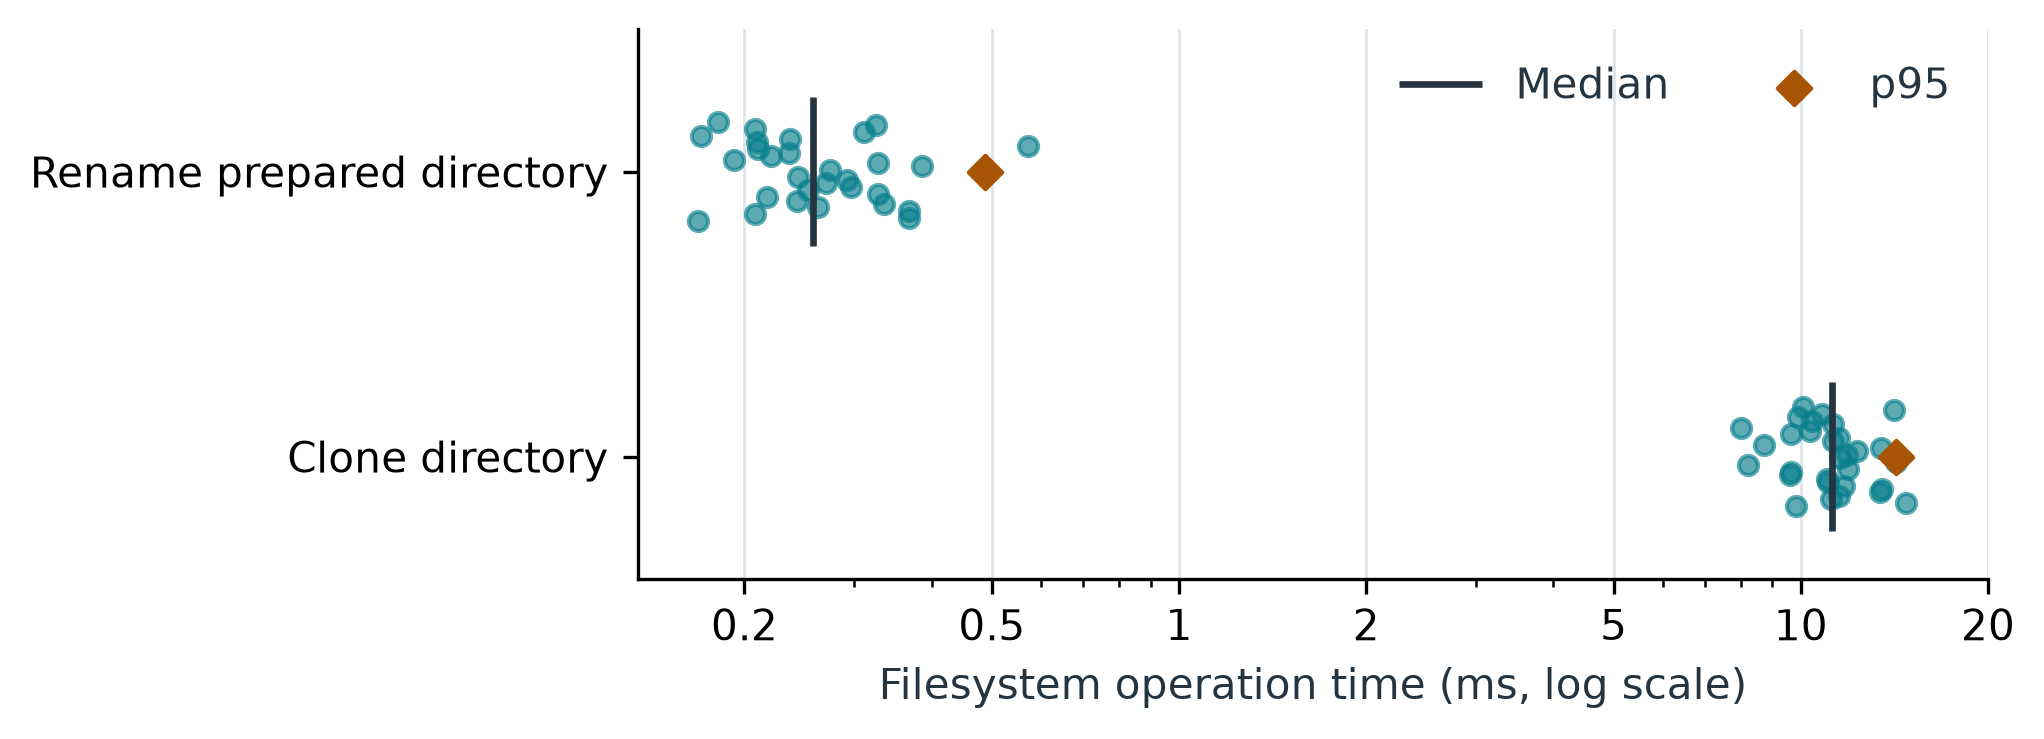
\includegraphics[width=1\linewidth,height=\textheight,keepaspectratio,alt={Thirty
timings per APFS operation on a logarithmic scale. Bars show medians and
diamonds show p95. Slot preparation and verification are outside the
timer.}]{paper-figures/replay-apfs-primitives.png}
\caption{Thirty timings per APFS operation on a logarithmic scale. Bars
show medians and diamonds show p95. Slot preparation and verification
are outside the timer.}
\end{figure}

\section{Threats to Validity}\label{threats-to-validity}

The reference model isolates one live-tree deletion and assumes a stable
sibling. It does not exercise the implementation's concurrent processes.
The APFS fixture contains synthetic regular files on one host. It
neither represents arbitrary npm layouts nor establishes power-loss
behavior. The historical install report does not archive every raw warm
repetition. The baseline differed across launch paths. The follow-up
checks the shared verifier and launcher proof with focused fixtures.
These limits bound the claim to the stated layout contract and the
measured conditions.

\section{Conclusion}\label{conclusion}

The fix was to stop copying from the directory users were about to
delete. A stable sibling removes that dependency and gives the worker a
source it can finish reading. Moving a ready slot to the project path
can reduce foreground publication time, while verification and
replacement of the consumed slot still incur work. A complete evaluation
should test each entrypoint against the same adversarial layouts and
compare end-to-end latency, hit rate, and deferred work across
filesystems.

\section*{Artifact Availability}\label{artifact-availability}
\addcontentsline{toc}{section}{Artifact Availability}

Run the \href{../../scripts/bench/paper_evidence.py}{evidence script}
with Python 3 to check the finite model and recompute the archived APFS
summaries. The optional --measure-apfs-primitives flag repeats the
synthetic test on macOS/APFS. The \href{../../LICENSE}{repository
license} governs the software.

\section*{References}\label{references}
\addcontentsline{toc}{section}{References}

\begin{enumerate}
\def\labelenumi{\arabic{enumi}.}
\tightlist
\item
  Bazel. ``Remote Caching.''
  \href{https://bazel.build/remote/caching}{Technical documentation}.
\item
  E. Dolstra. \emph{The Purely Functional Software Deployment Model}.
  PhD thesis, Utrecht University, 2006.
  \href{https://nixos.org/~eelco/pubs/phd-thesis.pdf}{Thesis}.
\item
  T. S. Pillai et al.~``All File Systems Are Not Created Equal: On the
  Complexity of Crafting Crash-Consistent Applications.'' \emph{USENIX
  Symposium on Operating Systems Design and Implementation}, 2014.
  \href{https://www.usenix.org/conference/osdi14/technical-sessions/presentation/pillai}{Paper}.
\end{enumerate}


\section*{Post-publication corrections (measured)}

\textbf{The reuse theorem needs two hypotheses it does not state.} Both come from incidents where
the mechanism silently did nothing or did the wrong thing:

\begin{enumerate}
\item \textbf{Freshness must be computed on final bytes.} The capsule marker was computed before the
lockfile was rewritten, so it never matched a tree that had just been installed: the mechanism was
unreachable, and every install re-resolved. A fingerprint over an input that later changes is a
fingerprint of the wrong object.
\item \textbf{A capsule must never be built from a directory the caller will delete.} The refill
cloned the live \code{node_modules}; the next wipe deleted it mid-clone, so every second run
discarded its slot. Refilling from a \emph{sibling} slot, and verifying the slot rather than the
live tree, fixed it.
\end{enumerate}

\textbf{Measured, macOS arm64, 71-package fixture.} Warm install 8--19\,ms (bun 26--32\,ms);
restore by \code{rename} 0.2--0.3\,ms; verification 3.4\,ms. A completion marker proves a write
finished, not that it produced anything: content is checked beside every ``already done'' test.


\section{Post-publication corrections: peer edges and platform identity (measured)}

Three defects shared one cause: \emph{a tree fact inferred from the wrong evidence}. Each is recorded
with the measurement that found it, because in every case the tree looked correct while its own plan
disagreed.

\begin{enumerate}
\item \textbf{Peer edges were advisory, not structural.} Installing \texttt{@testing-library/react\@14}
left \texttt{@types/react-dom} in the tree without its peer \texttt{@types/react}. The resolver
detected the requirement and printed ``got absent'' --- so the graph knew and the layout did not. A
post-pass over resolved instances cannot repair this: an instance that no edge refers to never
reaches the layout. The correction is that peers are \emph{demands}, queued at the same point as
dependencies so the ordinary edge bookkeeping places them.
\item \textbf{Optional peers are not demands.} Queueing every peer made \texttt{ts-node}'s optional
peers \texttt{@swc/core} and \texttt{@swc/wasm} real packages. The lockfile then listed
\texttt{@swc/wasm}, the layout refused it as a WebAssembly build, and \texttt{verify} failed with
\texttt{node_modules/@swc/wasm is missing} --- the tree contradicting its own plan. Optionality is
\texttt{peerDependenciesMeta}, and it must be read before the demand is queued, not after.
\item \textbf{Platform identity is declared metadata, never a name.} The materialisation filter
rejected packages by tokenising their names, and \texttt{@swc/wasm} contains the token \texttt{wasm}.
The package is real, is installed on every platform, and was silently dropped from trees that listed
it. The asymmetry settles the rule: skipping a loadable package breaks a tree, installing an
unloadable one wastes bytes. Only \texttt{os}/\texttt{cpu}/\texttt{libc} fields may exclude an entry,
which is why npm writes them. Name-token inference survives only where no fields exist at all.
\end{enumerate}

One measurement worth keeping: the first run after the metadata fix still dropped the entry, because
parsed lockfile entries are cached in a binary keyed by lockfile content and platform \emph{only}. A
cache keyed by its input alone will happily return answers produced by an older decision procedure,
so the key must carry the rule version.


\section{Post-publication correction: a lockfile states intent, not just an answer}

Measured on a real tree, the writer emitted \textbf{55 empty \texttt{dependencies} maps out of
70 entries} and pinned the rest to wired versions. Two rules follow, and both are about what a
lockfile \emph{is}.

First, every field that describes a package is \emph{declared} metadata: dependencies, optional
dependencies, peers, peer optionality, platform. It is copied from the published version document
by one constructor, never assembled by hand, because a hand-built entry at forty sites is forty
chances to write an empty map.

Second, a writer may consult a cache but must never derive its content from one. The lookup was
TTL-gated at sixty seconds, so two entries of the same file disagreed about the same question:
\texttt{accepts} came out correct and \texttt{express} came out empty because its packument had
aged out. A published version is immutable --- only \texttt{dist-tags} and \texttt{time} move ---
so the immutable half is read without a freshness window, and the lookup is a \emph{fallback}:
a miss must not erase edges the tree already knows.

Result: 68 of 69 entries match npm's dependency maps byte for byte. The exception is an optional
dependency recorded in \texttt{dependencies} rather than \texttt{optionalDependencies}, because
the entry type has no optional-edge class; that is a stated gap, not an unmeasured one.


\section{Post-publication correction: what a lockfile entry must contain}

After `dependencies` became declared ranges, the entry \emph{shape} still disagreed with npm. The
measurement was done field for field on a real tree, and it took three rounds:

\begin{center}
\begin{tabular}{lcl}
identical entries & change & why \\
\hline
0 / 69 & -- & empty \texttt{dependencies} maps, no \texttt{license} \\
48 / 69 & facts carried on the entry & a writer must not derive facts from a cache \\
68 / 69 & \texttt{license} retained by pruning & a version fact that the prune removed \\
69 / 69 & install-script checks all three hooks & \texttt{esbuild} works in \texttt{postinstall} \\
\end{tabular}
\end{center}

Two principles follow. First, \textbf{facts travel with the entry}: every declared field is copied
from the published version document once, at construction, and read from the entry afterwards.
Second, \textbf{optionality is a class, not a merge}: optional edges belong under
\texttt{optionalDependencies} and must not be copied into the required set, which is precisely what
made the last entry differ.

\end{document}
